\documentclass[11pt,  oneside, openany]{book}
\usepackage[greek, italian]{babel}
\usepackage{geometry}
\usepackage{float}
\usepackage{graphicx} 
\usepackage{array}
\usepackage{multirow}
\geometry{a4paper} 
\usepackage{listings} % necessario per inclusione codice sorgente
\usepackage{color} % syntax highlighting
\usepackage{url}
\usepackage{pdfpages}
\usepackage{caption}


\newcommand{\source}[1]{\caption*{Fonte: {#1}} }

% \textit {f}  
% ~, `` ''
% Controllare poi che i capitoli e paragrafi citati siano corretti. (es vedi Capitolo 4)

\pdfinfo{
   /Author (Rita Folisi)
   /Title  (Elaborato finale)
 
}

\title{Elaborato finale}
\date{}
\author{Rita Folisi}

\begin{document}
	\pagenumbering{gobble}

  \begin{titlepage}
    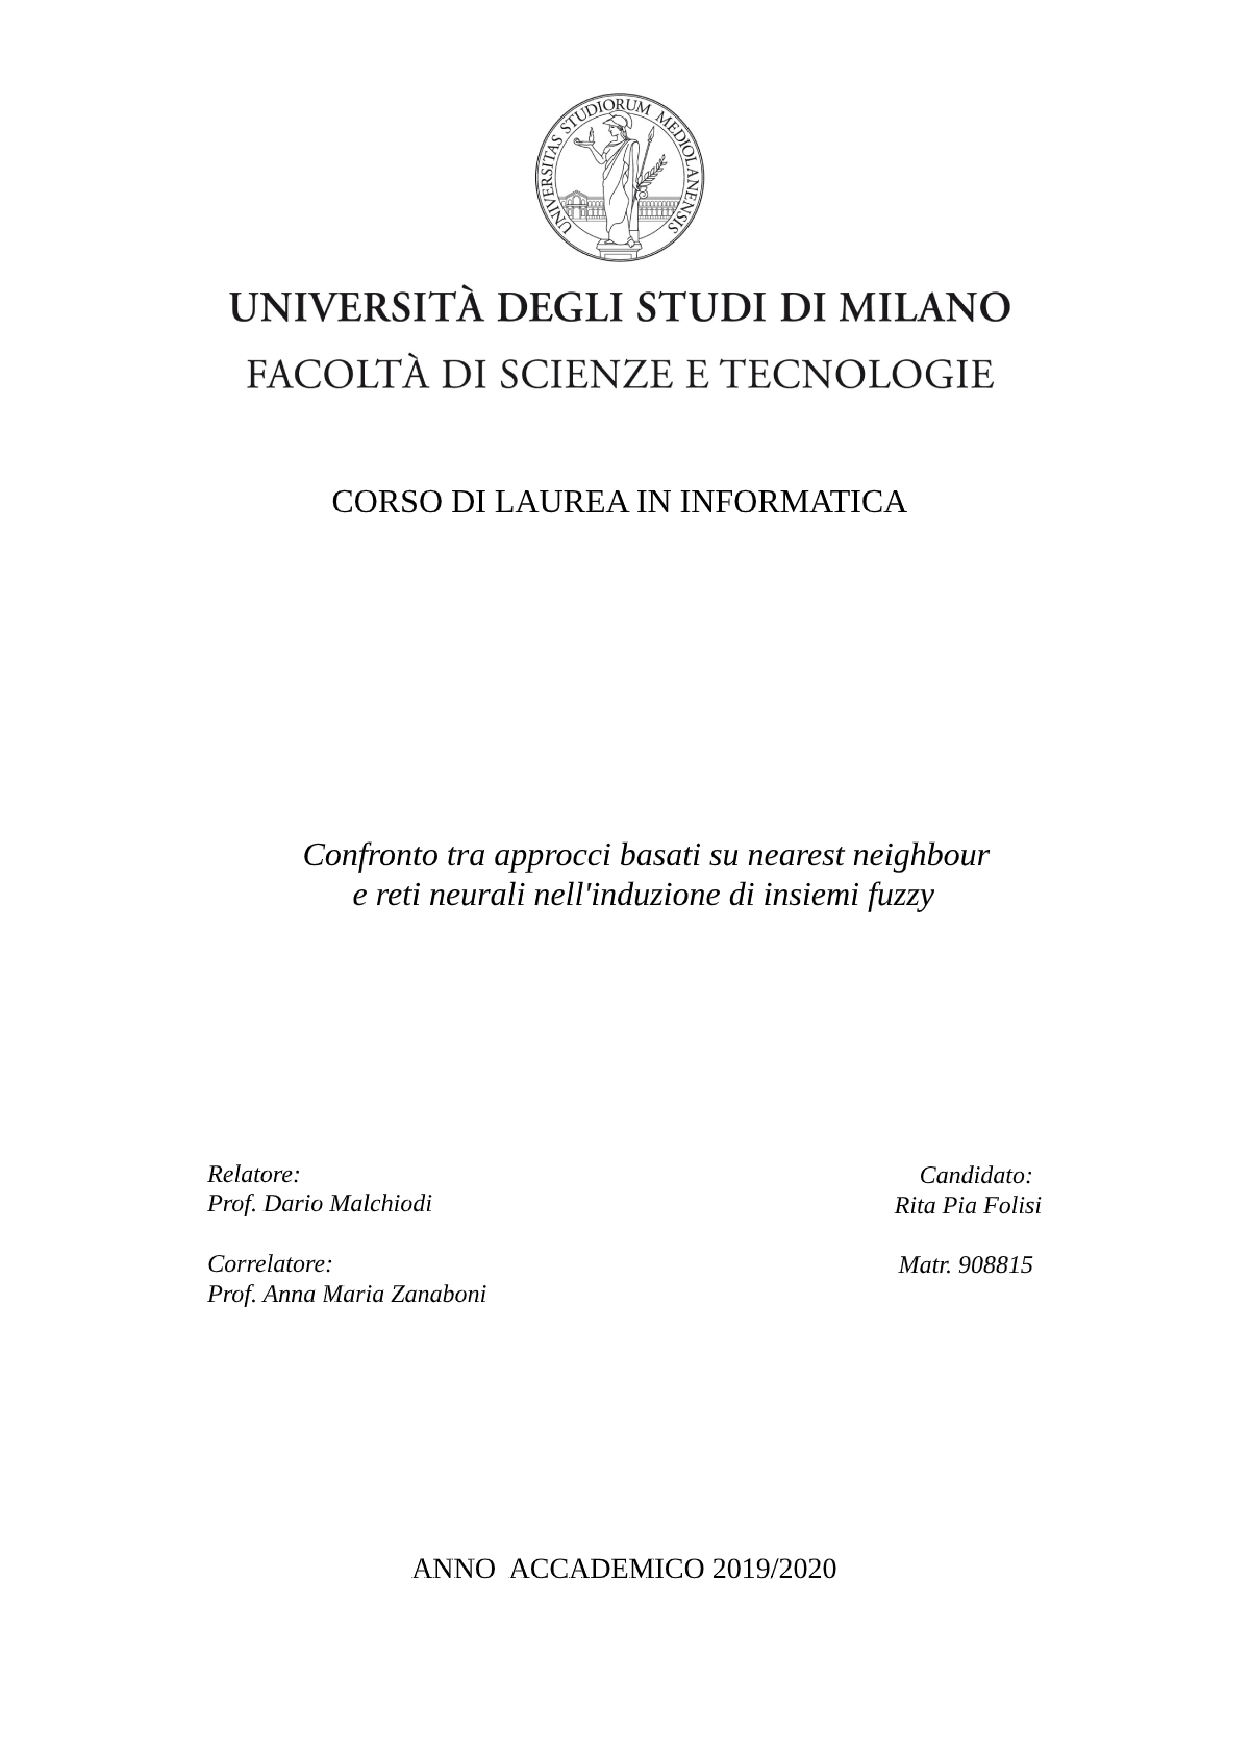
\includepdf{Immagini/Frontespizio.pdf}
    \tableofcontents
    \thispagestyle{empty}
  \end{titlepage}



	\pagenumbering{arabic}

	\chapter{Introduzione}

	\chapter{Apprendimento automatico e logica fuzzy}
Nel seguente capitolo si passano in rassegna i concetti di apprendimento automatico e di logica fuzzy, illustrando come i due argomenti possano essere coniugati insieme. Nel Paragrafo 2.1 ci si soffermerà sull'apprendimento supervisionato, di cui i metodi proposti in seguito faranno parte. Nel Paragrafo 2.2 si riprenderanno i concetti relativi ai \textit {fuzzy set}, fino a illustrare cosa significa indurne la funzione di appartenenza. 

	\section{Apprendimento supervisionato}

Con apprendimento automatico si intende l'abilità di una macchina di apprendere in maniera autonoma a partire da dati o da osservazioni, attraverso diversi algoritmi. A partire da questi dati la macchina impara una funzione, che permette attraverso di risolvere generiche istanze di un fissato problema. Nel seguito, sarà utilizzato il termine ``esempio'' per riferirsi ai dati sopracitati. In genere, vengono considerate varie classi di problemi, quali la classificazione, la regressione e il clustering. 

Da un punto di vista formale~\cite {mlstanford} si considerino un problema di riferimento, delle istanze di un problema e una funzione  $f$, che codifica la soluzione delle istanze del problema. Le istanze del problema sono descritte da un vettore  $X$ = $x_1...x_n$ composto da $n$ elementi e sono associate tramite la funzione $f$ ognuna alla propria soluzione. La funzione $f$ non è nota, ma si utilizza una funzione $h$ che la approssima al meglio\footnote{`E bene precisare che la bontà di tale approssimazione è legata alla metrica, la cui scelta non è una questione banale, come si vedrà in seguito}.  Le funzioni \textit {f} e \textit {h} sono definite sul vettore $X$ descritto precedentemente. Viene assunto a priori che \textit {h} viene selezionata da una classe di funzioni \textit {H}, alla quale \textit {f} può appartenere.  All'interno della classe di funzioni, \textit {h} viene scelta in base a $\Xi$, un insieme contenente $m$ esempi di apprendimento. Una volta scelta, \textit {h} viene implementata da una macchina, che avrà dunque input X e in output \textit {h}(X). 

L'apprendimento automatico può essere principalmente di due tipi: si parla, infatti, di modalità supervisionata e non supervisionata. In questo elaborato, tuttavia, verrà trattato soltanto l'apprendimento supervisionato, in cui l'insieme $\Xi$ contiene le coppie input-output della funzione \textit {f}. 
Se il processo di apprendimento riesce a selezionare una funzione \textit {h} che approssima bene \textit {f} per i valori di $\Xi$, allora si può ipotizzare che \textit {h} sia un'ottima approssimazione per \textit {f} anche in generale. In altri termini, attraverso esempi di apprendimento costituiti da coppie di input e di output, viene costruito il modello, cioè una funzione capace di fornire buone predizioni in relazione a nuovi input. 
Quando tale output è rappresentato da una variabile discreta si parla di classificazione, se invece è una variabile continua si parla di regressione. Il campo esaminato durante il tirocinio riguarda i problemi di classificazione e pertanto l'obiettivo dei metodi presentati in seguito sarà, dato un vettore di input, fornire una predizione sperabilmente corretta. Gli output possono anche essere definiti come $label$ o etichetta. D'altra parte, il vettore di input $X$ può essere definito anche come \textit {feature vector} e le componenti $x_i$ \textit come {feature} o attributi, i cui valori possono essere di tre tipologie: numeri reali, discreti o valori categorici.
Un esempio di problema di classificazione è il filtraggio anti-spam. In questo caso, gli esempi di addestramento avranno come vettore $X$  il contenuto testuale e i metadati di ogni mail, mentre come etichetta un bit che dichiara se il messaggio sia spam o meno.

Una volta addestrato il modello con gli esempi di apprendimento, occorre valutare le performance per comprendere se questo è in grado di eseguire correttamente il suo compito. In funzione del problema da affrontare, si adottano criteri diversi: nel caso della classificazione si utilizza in genere l'accuratezza, mentre nella regressione si  usano funzioni di errore. L'accuratezza è il numero di predizioni corrette divise per il totale delle predizioni effettuate e viene espresso in percentuale. 

Tra le funzioni di errore, è molto comune l'errore quadratico medio (\textit{mean square error}), che quantifica quanto le predizioni eseguite dal modello siano vicine all'etichetta attraverso questa formula: 

$$MSE = \frac{1}{n}\sum_{i=1}^{n}(y_{i} - h(x_{i}))^{2}$$, 
dove $y_i$ è l'etichetta, mentre $h(x_{i})$ è la predizione effettuata dal modello. 
Un'altra funzione di errore utilizzata è RMSE ovvero la radice quadrata dell'errore quadratico medio: 

$$RMSE = \sqrt{\frac{1}{n}\sum_{i=1}^{n}(y_{i} - h(x_{i}))^{2}}$$. 

In genere, alla funzione di errore si affianca anche una soglia, che precisa quale il margine di errore è considerato accettabile. Le funzioni di errore in realtà  possono essere utilizzate anche con problemi di classificazione, ma l'accuratezza non viene utilizzata mai con problemi di regressione. 
La valutazione non viene effettuata sugli esempi utilizzati per l'apprendimento, dal momento che l'obiettivo del modello è generalizzare con dati diversi da quelli osservati in precedenza. Dati degli esempi del problema che si vuole risolvere, occorre distinguere una parte di dati dedita ad addestrare il modello (\textit{training set}) e un'altra dedita a valutarne la prestazione (\textit{testing set}). Il primo verrà utilizzato in fase di apprendimento, mentre il secondo verrà utilizzato esclusivamente alla fine per decretare le performance del modello. I due set possono presentare delle criticità tali da poter alterare l'intero processo di apprendimento e valutazione. Ad esempio, possono avere una dimensione molto elevata di feature, comportando un aumento della complessità computazionale dell'algoritmo di apprendimento; per risolvere questo problema, si utilizzano algoritmi di selezione delle feature, con lo scopo di selezionare quelle più rilevanti per migliorare le predizioni e le performance generali. Un'altra criticità è causata dal rumore nei dati. Nel caso sia presente nei dati di training, il rumore di classe altera i valori di \textit{f}, mentre il rumore di attributo altera i valori delle componenti dei vettori di input, compromettendo dunque la corretta associazione input-output. Inoltre, è bene osservare quanto il training set sia rappresentativo del campo in analisi: infatti, può accadere che questo presenti poca varietà e che il metodo dunque non sia in grado di generalizzare. Ad esempio, se nel training set sono presenti, sotto la label di ``orologio'', solo immagini di orologi rotondi e di color rosso, quando il modello si ritroverà a dover predire la label di un orologio quadrato e giallo probabilmente non darà la risposta corretta. Questo fenomeno prende il nome di \textit {overfitting} ed è facilmente visibile quando il modello si adatta molto ai dati di training ma riporta performance sensibilmente inferiori con i dati di testing. 

\begin{figure}[h!]
\begin{center}
  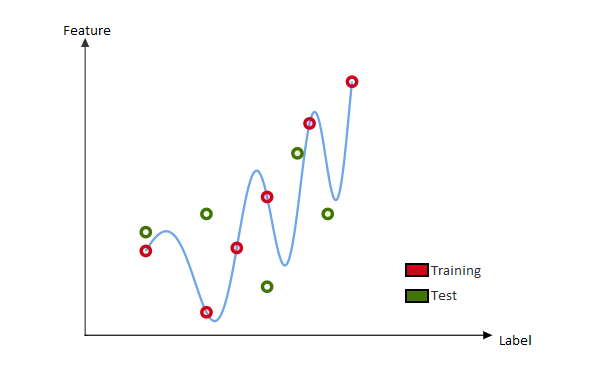
\includegraphics[width=13cm]{Immagini/Overfitting.png}\\
  \caption{Illustrazione grafica del fenomeno dell'overfitting}
\end{center}
\end{figure}

Graficamente, si avrà la situazione presente in Figura 2.1, ovvero la funzione in blu $h$, appresa dal modello, si adatterà perfettamente ai dati di training (segnati in rosso), ma non riuscirà a predire bene i dati di testing. In altri termini, se il modello allenato viene eseguito sui dati di training, il modello produrrà un numero sensibilmente minore di errori rispetto a quando viene eseguito sui dati di testing. Un overfitting può essere causato anche da una suddivisione casuale dei dati che comporti l'inserimento nel training set di osservazioni non generali. Più in generale, nel valutare le performance, è bene considerare quanto la scelta di determinati esempi di apprendimento possa influenzare le performance. Può infatti succedere che una buona valutazione sia data da una scelta fortuita di esempi di apprendimento, mentre con un'altra scelta di esempi tale modello non dia la stessa performance. Dunque la valutazione effettuata dopo aver allenato il modello è la valutazione di un solo esperimento, non per forza del modello in sé. Occorre dunque uno strumento che possa generalizzare le valutazioni delle performance complessive di un modello. Per la risoluzione del problema, si rimanda ai paragrafi successivi. 


Normalmente, prima di effettuare il processo di apprendimento, occorre impostare uno o più iperparametri. Si definiscono iperparametri tutte le parti del modello da impostare prima di iniziare la fase di apprendimento, mentre i parametri sono quelle parti del modello apprese durante la fase di apprendimento. Impostare gli iperparametri non è un'operazione semplice, dal momento che una configurazione erronea può incidere notevolmente sulle performance del modello. Si parla pertanto di \textit{model selection} (selezione del modello) o \textit{tuning degli iperparametri}, che si servono di un sottinsieme del training set, che prende il nome di \textit{validation set}. L'obiettivo è trovare la combinazione di iperparametri che ottimizza le performance del modello. Si definiscono gli insiemi di valori potenziali di ogni iperparametro e il modello viene addestrato con tutte le combinazioni possibili. Si decreta poi il \textit{validation score} (punteggio di validazione), che è coerente con il criterio scelto per valutare le performance del modello alla fine. Infine, si selezionano i parametri che massimizzano il validation score e vengono assegnati al modello. 
 

Per risolvere il problema della model selection e della generalizzazione delle valutazioni, si ricorre alla \textit{k-fold cross validation}. Più in generale, la cross validation è una tecnica utilizzata per la suddivisione del dataset in training set e in validation set nel primo caso o in training set e in testing set nel secondo caso. Si prenda ad esempio il problema della model selection e quindi della suddivisione in training set e in validation set. Si definisce il numero di fold \textit{k} e si divide il dataset $\Xi$ in \textit{k} sottinsiemi mutuamente esclusivi e di ugual dimensione: $\Xi_1 ... \Xi_k$. In seguito, si reitera l'algoritmo di apprendimento \textit{k} volte considerando a ogni iterazione il sottinsieme $\Xi_k$ come training set e i rimanenti come validation set. La valutazione finale viene effettuata facendo la media delle valutazioni parziali dei sottinsiemi. In Figura 2.2 è presente una visualizzazione grafica della cross validation, con suddivisione in training set e validation set. Tale procedimento è del tutto analogo anche nel caso in cui si voglia generalizzare le valutazioni delle performance e dunque suddividere in training set e testing set. Qualora si volesse risolvere in maniera combinata entrambi i problemi, sarà necessario fare una crossvalidation annidata nell'altra. Per maggiori dettagli implementativi si rimanda al Capitolo 4. 

\begin{figure}[h!]
\begin{center}
  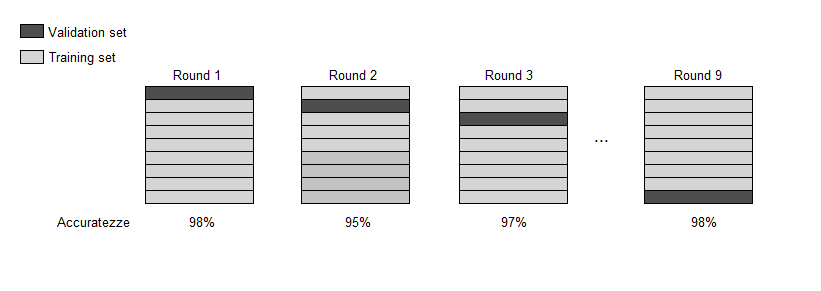
\includegraphics[width=13cm]{Immagini/Crossvalidation.png}\\
  \caption{Cross validation}
\end{center}
\end{figure}

	\section{Logica fuzzy e fuzzy set}
Il linguaggio e il ragionamento umano, spesso imprecisi e complessi, difficilmente sono colti appieno dalla logica classica basata sull'assegnazione di un valore di verità binario (vero o falso). Infatti, nel linguaggio naturale, molte espressioni risultano ambigue e, per la loro mancanza di formalità, diventano difficilmente trattabili con i classici strumenti della matematica. Una proposizione, in particolare, viene definita imprecisa nel momento in cui contiene predicati che possono essere veri o falsi solo parzialmente o solo a un certo grado. Un esempio concreto è la frase ``Il caffè è abbastanza dolce''. In questa frase il concetto di dolce non è formalizzato e non ha un significato fisso, in quanto non viene indicata una certa quantità di zucchero affinché il caffè possa considerarsi effettivamente dolce. Inoltre, è accompagnata dall'avverbio ``abbastanza'', che non esprime a sua volta un grado di certezza ben definito. Pertanto, alla proposizione è impossibile affidare un valore di verità binario, dal momento che il grado di dolcezza è soggettivo e, dunque, non interpretabile universalmente. Per poter trattare queste situazioni si introduce la \textit{logica fuzzy}~\cite{fuzzylogicintro}, un'estensione della logica booleana. La logica fuzzy attribuisce ad ogni proposizione un valore di verità compreso tra 0 e 1, estremi inclusi: pertanto, è capace di trattare proposizioni vere (valore pari ad 1), false (valore pari a 0) e parzialmente vere o false (valore compreso tra 0 e 1). Permettendo quindi alle proposizioni di trovarsi in uno stato diverso dal vero o falso, la logica fuzzy consente di descrivere con flessibilità il ragionamento umano e gestire l'incertezza e l'inesattezza. Per questo motivo è ampiamente utilizzata in molti domini di applicazione, come processi decisionali, analisi testuale, \textit{data analysis}, \textit{feature extraction} in un'immagine. Un esempio recente di applicabilità è stato presentato in ~\cite{fuzzybraintumor}, dove vengono elaborate immagini di risonanze magnetiche del cervello per poterne rilevare anomalie. 

\subsection{Fuzzy set e funzione di appartenenza}
Il \textit{fuzzy set} è una generalizzazione della teoria classica degli insiemi e si basa sulla logica fuzzy. Viene definito come un raggruppamento di oggetti ed è caratterizzato da una funzione che sintetizza il grado di appartenenza di ogni oggetto all'insieme stesso. Formalmente, si avranno un universo del discorso $X$, un generico elemento $x$  appartenente a $X$ e un generico fuzzy set $A$ contenuto in $X$. L'insieme $A$ è caratterizzato da una funzione $f_A$, che prende il nome di \textit{membership function}, che associa a ogni punto $x$ un numero reale dell'intervallo [0,1]. Il valore $f_A(x)$ rappresenta il grado di appartenenza (\textit {membership value}) di $x$ ad $A$. Più questo valore sarà prossimo a 1, maggiore sarà il grado di appartenenza di $x$ ad $A$. Quindi 1 indicherà la piena appartenenza all'insieme $A$, mentre 0 indicherà la piena esclusione. I valori compresi tra 1 e 0 indicheranno invece la parziale appartenenza all'insieme $A$. Gli insiemi classici possono essere visti come un caso particolare di fuzzy set, dove gli unici valori di membership ammessi sono 1 e 0, corrispondenti a piena appartenenza o piena esclusione. Questo tipo di insiemi prende il nome di \textit{crisp set} o \textit{boolean set} e $f_A(x)$ avrà solo valori 0 o 1 (vedi Figura 2.3). 


\begin{figure}[h!]
\begin{center}
  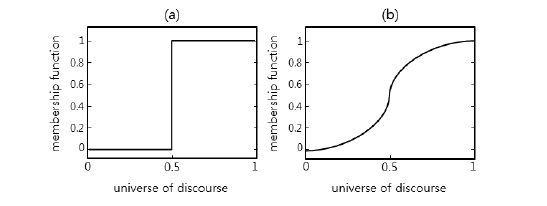
\includegraphics[width=13cm]{Immagini/membfunctcrispvsfuzzy.png}\\
  \caption{Membership function di un crisp set e di un fuzzy set}
  \source{\url{https://www.researchgate.net/figure/Membership-function-with-Crisp-seta-and-Fuzzy-setb-Walczak-and-Massart-1999_fig1_264167589} [Accesso in settembre 2020]}
\end{center}
\end{figure}

In Figura 2.4 è possibile osservare la rappresentazione grafica di un crisp set (a sinistra) e di un fuzzy set (a destra). Il crisp set ha i contorni ben delineati e presenta due soli colori, bianco o nero: ciò accade poiché un punto può o appartenere al set e quindi trovarsi nello spazio in nero, oppure non appartenere al set e dunque trovarsi nello spazio bianco. Il fuzzy set, invece, avrà i contorni più sfumati e zone in grigio, dal momento che contempla l'imprecisione e l'incertezza e pertanto un punto può parzialmente appartenere a un insieme. 

\begin{figure}[h!]
\begin{center}
  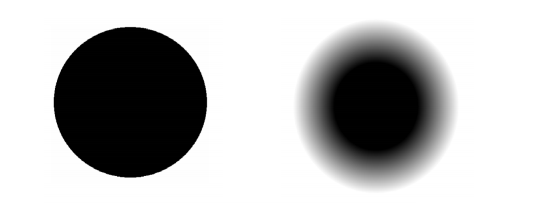
\includegraphics[width=13cm]{Immagini/fuzzyvscrisp.png}\\
  \caption{Rappresentazione grafica di un crisp set e di un fuzzy set}
\end{center}
\end{figure}


% Si può inserire volendo un paragrafo che parla di operazioni su insiemi fuzzy

\subsection{Variabile linguistica e FIS}

% fonte: http://groups.di.unipi.it/~cappelli/seminari/falotico.pdf

Un altro concetto sul quale si basa la logica fuzzy è quello di variabili linguistiche, attraverso cui è possibile avvicinarsi al linguaggio naturale. Infatti, una variabile linguistica ha come valori attributi linguistici, ovvero parole utilizzate nel linguaggio naturale: in particolare, si potranno generare variabili da termini primari (ad esempio ``alto''), modificatori (avverbi come ``molto'', ``sicuramente'', ``abbastanza'' etc.)  e connettori (``e'', ``o'', ``non''). Secondo la definizione di Zadeh, una variabile linguistica viene definita come una quintupla $(V, T(V), U, G, M)$ dove: 

\begin{itemize}
\item $V$ è il nome della variabile linguistica, 
\item $T(V)$ è l'insieme dei termini dei valori linguistici della variabile $V$ (\textit{term set}), 
\item $U$ è l'universo del discorso, cioè il dominio in cui sono definite le variabili, 
\item $G$ è la regola sintattica che genera i nomi in $T(X)$ applicando modificatori linguistici ai termini primari, 
\item $M$ è la regola semantica che assegna a ciascun nome il suo significato, cioè un insieme fuzzy attraverso una funzione di compatibilità $c : U \to [0,1]$. 
\end{itemize}

Ad esempio, data una variabile linguistica $X$ = età, avremo come universo $U$ l'intervallo dei valori assumibili da $X$, ad esempio U=[0, 122]. Un insieme $T(X)$ può essere ''vecchio, molto vecchio, giovane, poco giovane''. La regola $G$ genera nomi applicando modificatori linguistici (``molto'', ``poco'') ai termini primari (``vecchio'', ``giovane''). Infine, la regola $M$ assegnerà ad esempio al valore 27 all'etichetta ``giovane'' con un grado di 0.7. I modificatori, divisi in varie categorie come quelli di concentrazione, di dilatazione e di contrasto, riescono così a rimodellare la regola semantica M, di modo da poter rispecchiare e rappresentare la vaghezza caratterizzante il linguaggio naturale. 

Le variabili linguistiche possono essere utilizzate all'interno dei FIS (\textit{fuzzy inference systems})~\cite{fis}, che consentono il mapping tra input-output crisp attraverso funzioni di appartenenza, operatori logici e regole fuzzy. I FIS vengono utilizzati per classificazione, problemi decisionali, ragionamento approssimativo e altro. Si avvalgono di un processo di fuzzificazione(\textit{fuzzification})~\cite{fuzzific}, cioè di costruzione di un insieme fuzzy a partire da valori di una data variabile, e di defuzzificazione (\textit{defuzzification}), che trasforma un insieme fuzzy in un valore numerico. La fuzzificazione è dunque la fase in cui si determina il grado con cui ogni input appartiene ad ogni fuzzy set; per far ciò, ci si avvale della funzione di appartenenza. 

\subsection{Apprendimento automatico supervisionato e fuzzy set}

Per molto tempo, all'interno della teoria dei fuzzy set, grande peso ha assunto la rappresentazione della conoscenza, soprattutto in relazione allo sviluppo di sistemi intelligenti e intelligenza artificiale. Tuttavia, negli ultimi anni sono emersi sempre più problemi con l'approccio puramente \textit{knowledge-driven}, che si basa sull'utilizzo da parte di un sistema di inferenza di conoscenze definite a priori, dal momento che risulta essere difficoltoso, intricato e spesso poco produttivo in termini di risultati. Di conseguenza, si è pensato di adattare i concetti della teoria dei fuzzy set a un approccio \textit{data-driven}, che invece utilizza i dati empirici per estrarre modelli. In questo modo, dunque, si può osservare come la teoria dei fuzzy set sia stata applicata all'interno dell'apprendimento automatico supervisionato, portando così alla nascita della \textit{fuzzy machine learning}~\cite{fuzzyml}. Difatti, la teoria dei fuzzy set riesce a rispondere a problemi di analisi dei dati, risultando pertanto un ottimo strumento per l'ambito dell'apprendimento automatico supervisionato. Difatti, la logica fuzzy risulta idonea, ad esempio, per operare con la vaghezza risultante dai dati empirici, che risentono di linguaggio naturale~\cite{fuzzydata}. 
Gli algoritmi classici del machine learning vengono pertanto estesi ai corrispettivi fuzzy: saranno presenti dunque alberi di decisione fuzzy~\cite{fuzzydectree}, fuzzy clustering~\cite{fcm-intro}, fuzzy k-nearest neighbors~\cite{fknn-example1} e così via. In Figura 2.5 è presente un esempio di albero di decisione fuzzy. In questo modo è dunque possibile combinare punti di forza dei metodi classici e della teoria fuzzy al fine di ottenere un metodo che riesce ad ottimizzare caratteristiche del modello altrimenti più complessi da migliorare, come l'interpretabilità dei dati e la gradualità. 

\begin{figure}[h!]
\begin{center}
  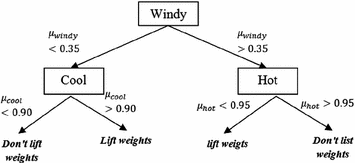
\includegraphics[width=10cm]{Immagini/fuzzyTreeDecis.png}\\
  \caption{Esempio di albero di decisione fuzzy}
\end{center}
\end{figure}

Relativamente al fuzzy machine learning, il focus di questo elaborato è l'induzione di funzioni di appartenenza, cioè la produzione di modelli che, date variabili in input, riescano a predire i gradi di appartenenza a insiemi fuzzy. In generale la costruzione della funzione di appartenenza può essere effettuata attraverso metodi deduttivi e induttivi. I primi sono knowledge-driven, mentre i secondi presentano un approccio data-driven. Nel prossimo capitolo ci si soffermerà su algoritmi induttivi, con il fine di risolvere problemi di classificazione attraverso l'induzione della funzione di appartenenza. 


	\newpage
	\chapter{Tecniche per l'induzione della funzione di appartenenza}

Generare la funzione di appartenenza dato un particolare problema è un compito piuttosto complesso all'interno della teoria della logica fuzzy, dovuto all'interpretazione che si può attribuire al concetto di funzione di appartenenza. In particolare, Dubois e Prade~\cite{membinterp} affermano che vi possano essere tre interpretazioni differenti della questione, comportando dunque l'inesistenza di regole generali e sempre ottimali per la generazione della funzione di appartenenza. Ad esempio, la frase ``Il valore di appartenenza di George Bush alla classe di uomini alti è 0.8''~\cite{membpaper} può essere vista in tre differenti modi:

\begin{enumerate}
\item Vista probabilistica: l'80\% della popolazione dichiara che George Bush è alto.
\item Vista dell'insieme casuale: l'80\% della popolazione definisce alto come un intervallo che comprende l'altezza di George Bush.
\item Vista di tipicità: l'altezza di George Bush presenta una distanza normalizzata pari a 0.2 dal prototipo più vicino al concetto di alto, che avrà invece grado di appartenenza pari a 1. 
\end{enumerate}

Non esistendo dunque un'interpretazione univoca, si può ben comprendere come i metodi deduttivi possano risultare inefficaci per stimare la funzione di appartenza, in quanto una stessa variabile può comportare interpretazioni diverse e dunque a funzioni di appartenenza diverse. Non esiste, in altri termini, un processo automatizzabile per la generazione della funzione che risponde perfettamente ad ogni situazione proposta. Per questo motivo, si utilizzano gli algoritmi induttivi che consentono una generalizzazione della funzione a partire da dati empirici, permettendo dunque di risolvere le ambiguità di interpretazione e di definire maggiormente il dominio. In generale in letteratura son stati presentati molti algoritmi, tra i quali si annoverano metodi basati sulla percezione, metodi euristici, clustering, support vector machine, istogrammi, k-nearest neighbour, reti neurali, algoritmi genetici e istogrammi. 
\`E bene notare che non esistono misurazioni che in generale sappiano decretare il metodo migliore per la generazione delle funzioni di appartenenza, ma varia in base al campo e al problema sui quali si opera. Ciò può risultare problematico nel momento in cui si cerca di modellare concetti che non hanno un significato concreto, ma puramente astratto: in tal caso è necessario che il modello utilizzato per indurre la funzione di appartenenza sia abbastanza flessibile e facilmente modificabile, per poter migliorare le performance generali dell'algoritmo. La generazione della funzione di appartenenza diviene così uno passaggio abbastanza cruciale, dal momento che influenza anche le performance generali dell'algoritmo scelto. La scelta di un metodo a dispetto di un altro risulta dunque fortemente legata al tipo di problema e al tipo di dati ai quali ci si interfaccia. 

In questo capitolo, si illustreranno nel paragrafo 3.1 i metodi basati sulle reti neurali e nel paragrafo 3.2 i metodi basati sull'algoritmo di k-nearest neighbour. In entrambi i capitoli si illustrerà il funzionamento degli algoritmi proposti e si darà una panoramica generale delle possibili varianti. 

\newpage

	\section{Reti neurali}

Le reti neurali artificiali (ANN) sono modelli computazionali e matematici composti da neuroni artificiali, che traggono ispirazione dalle reti neurali biologiche del cervello umano. Difatti, come le reti neutrali celebrali permettono all'individuo di ragionare e di apprendere, le reti neurali artificiali apprendono attraverso una fitta rete di neuroni interconessi che rielaborano le informazioni e le spediscono poi ai neuroni successivi. Le reti neurali vengono ampiamente utilizzate in molteplici campi, tra cui riconoscimento di pattern (ad esempio in bioinformatica), classificazione e compressione di dati. Come è possibile vedere in Figura 3.1, le reti neurali presentano essezialmente tre tipologie di strati o \textit{layer}: un \textit{input layer}, che riceve dati in ingresso, diversi \textit{hidden layer}, che si occupano dell'elaborazione e un \textit{output layer}, che raccoglie i risultati dell'elaborazione. Il numero di nodi in input è pari al numero delle feature dei vettori di input, mentre il numero di nodi in output è pari al numero di etichette.  Ogni neurone di un layer può avere molteplici connessioni con i neuroni del layer successivo: ad esempio, , è possibile avere una rete neurale \textit{fully connected}). 

\begin{figure}[h!]
\begin{center}
  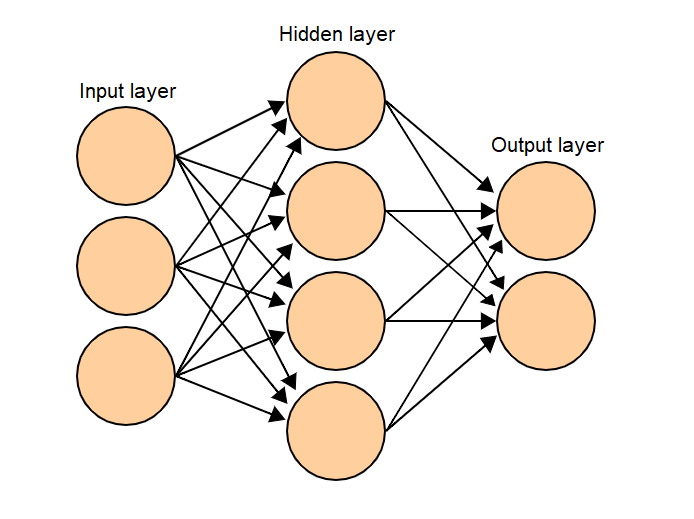
\includegraphics[width=10cm]{Immagini/ReteNeurale.png}\\
  \caption{Struttura di una rete neurale artificiale}
  \source{\url{https://commons.wikimedia.org/w/index.php?curid=1496812} [Accesso in Settembre 2020]}
\end{center}
\end{figure}

I neuroni e le connessioni tra neuroni presentano dei pesi da aggiustare durante la fase di apprendimento, per rafforzare o meno il segnale da mandare al neurone successivo. Spesso, all'interno del nodo vi è una soglia che decreta se tale segnale verrà trasmesso ai neuroni successivi o meno. Per determinare l'output di ogni neurone, si sommano tutti i pesi ricevuti in input, ognuno dei quali è composto dal peso del neurone del layer precedente moltiplicato per il peso della connessione associata. A questo peso si aggiunge un bias e il risultato finale viene dato in input a una funzione di attivazione che produce l'output da trasmettere ai neuroni del layer successivo. Infine, nell'output layer si raccoglie l'output finale. 
Le reti neurali vengono definite anche ``adattive'', dal momento che sono in grado di modificare la propria struttura e i propri pesi attraverso la rielaborazione dei dati esterni e delle informazioni interne, ottenuta durante la fase di apprendimento. Con l'approccio supervisionato, le reti neurali vengono addestrate attraverso esempi, di cui è anche nota l'etichetta. In questo modo, durante il processo di apprendimento, il modello confronta l'output predetto con l'etichetta reale e questa differenza, definita dalla funzione di perdita, verrà utilizzata per ridefinire i pesi interni. Infatti, una volta calcolata la funzione di perdita, si torna indietro nella rete per sistemare tutti i pesi e minimizzare così la funzione di costo. Per sistemare i pesi, si utilizza l'algoritmo di backpropagation, che sfrutta metodi di ottimizzazione come la discesa del gradiente. 



\subsection{Neurofuzzy}
Le reti neurali descritte sopra possono essere utilizzate per generare funzioni di appartenenza, dal momento che i valori di output della funzione di attivazione di ogni neurone sono simili ai valori di appartenenza dei fuzzy set. Una volta addestrata la rete, pertanto, questa può essere utilizzata per generare gradi di appartenenza, ricevendo in input il vettore delle feature e dando in output il grado di appartenenza ai fuzzy set. Questo approccio funziona dal momento che le funzioni di attivazione hanno la stessa forma di
alcune funzioni di appartenenza ~\cite{membneuralnetwsimilar}. Le reti neurali e i fuzzy system hanno delle caratteristiche abbastanza diverse tra loro, come è possibile vedere nella Tabella \ref{table:0}~\cite{neurofuzzyintro}. Entrambi i sistemi presentano i loro punti di forza e le loro debolezze. Da una parte, i sistemi fuzzy sono in grado di rappresentare l'incertezza, sono facilmente estendibili grazie alla generazione di nuove regole e risultano essere robusti, ma sono incapaci di generalizzare. D'altra parte, le reti neurali sanno apprendere e generalizzare, ma è più complesso interpretarle e determinare il numero di layer e neuroni ~\cite{surveyneurofuzzy}.


\begin{table}[h!]
\centering
\begin{tabular}{ |p{7cm}|p{7cm}| } 
\hline
\textbf{Reti neurali} & \textbf{Fuzzy System} \\
\hline
\hline
Sono strutture di basso livello & Affrontano ragionamento di alto livello\\ 
\hline
Buone performance quando sono si utilizzano molti esempi di apprendimento & Utilizzano informazioni linguistiche da esperti del dominio \\
\hline
Possono appredere & Non imparano e non si adattano a nuovi environment \\
\hline
Sono scatole nere per l'utente & Si basano sul linguaggio naturale\\
\hline

\end{tabular}
\caption{Differenze tra reti neurali e fuzzy system}
\label{table:0}
\end{table}

La loro combinazione consente di ottenere un sistema capace di integrare la capacità di apprendere delle reti neurali e la flessibilità vicina al ragionamento umano dei sistemi fuzzy. Tale sistema prende il nome \textit{neurofuzzy}, un modello ibrido in cui i fuzzy set e le regole vengono sistemate, in un vero e proprio processo di tuning, attraverso le tecniche delle reti neurali. 
Esistono diversi approcci al riguardo, di cui si fornisce una breve elencazione in seguito. 

\begin{itemize}
\item \textit{Cooperative Neuro-Fuzzy System}: esiste una fase di pre-processing in cui attraverso le reti neurali si determinano alcuni sottoblocchi del sistema fuzzy; in seguito, si esegue soltanto il sistema fuzzy. Ha come svantaggio che la struttura diventa non totalmente interpretabile. 
\item \textit{Concurrent Neuro-Fuzzy System}: la rete neurale e il sistema fuzzy lavorano insieme in modo continuativo. Generalmente, l'input entra nel sistema fuzzy, viene pre-processato ed in seguito viene immesso nella rete neurale, oppure si può invertire il processo. Uno svantaggio, tuttavia, è la minore interpretabilità dei risultati. 
\item \textit{Hybrid Neuro-Fuzzy System}: la rete neurale apprende alcuni parametri del sistema fuzzy in modo iterativo. Tra tutti è l'approccio più utilizzato. 
\end{itemize}

Nel terzo approccio il sistema complessivo riprende due modalità diverse. Dapprima, nella fase di apprendimento, impara i propri parametri interni come una rete neurale. In seguito, durante la fase di esecuzione, si comporterà come un sistema fuzzy. Questa scelta è stata adottata dal momento che esistono algoritmi efficienti di apprendimento presenti nelle reti neurali, che riescono dunque ad alleviare il processo di tuning dei sistemi fuzzy. Di questo approccio sono state fornite diversi modelli, che spesso risultano essere abbastanza simili tra loro. Una delle famiglie di architetture più comuni è ANFIS, di cui sono state registrate varianti in Tabella \ref{table:1}.

\subsection{Fuzzy min-max Neural Network}

Negli ultimi anni, la classificazione di pattern è diventata uno dei campi più importanti dell'intelligenza artificiale, dal momento che fornisce innumerevoli applicazioni nel mondo reale. In questo ambito, sia le reti neurali sia la logica fuzzy sono state ampiamente utilizzati, e pertanto si è deciso di costruire un modello ibrido che combina i due sistemi. 
L'algoritmo fuzzy min-max neural network utilizza i fuzzy set come \textit{pattern class}. L'idea è quella di avere una rete neurale che crea classi aggregando diversi fuzzy set più piccoli in un singolo fuzzy set, che corrisponderà alla classe. L'algoritmo si basa sulla costruzione di \textit{hyperbox}. Un hyperbox descrive una regione n-dimensionale definita completamente dai punti di minimo e di massimo, in corrispondenza dei quali viene definita la funzione di appartenenza. In Figura 3.2 è raffigurato un hyperbox, con associata una funzione di appartenenza che determina con quale grado un punto $x\in R^3$ è contenuto all'interno del box. La collezione di questi hyperbox forma un pattern class. 

\begin{figure}[h!]
\begin{center}
  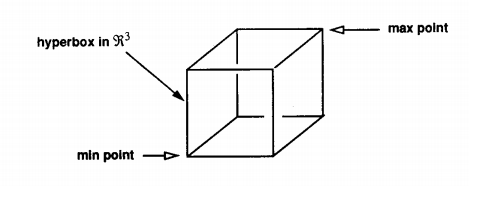
\includegraphics[width=10cm]{Immagini/hyperbox.png}\\
  \caption{Esempio di hyperbox}
\end{center}
\end{figure}

I punti di minimo e di massimo vengono determinati attraverso il \textit{fuzzy min-max learning algorithm}, un processo di espansione e contrazione che impara e definisce i confini dei fuzzy set e quindi delle classi. Ogni fuzzy set class è formato dall'aggregazione di più hyperbox, operazione svolta all'interno della struttura della rete neurale. L'apprendimento avviene collocando correttamente gli hyperboxes nel \textit{pattern space}. In seguito è stata fornita una breve descrizione dell'algoritmo fuzzy min-max learning: 

\begin{itemize}
\item Espansione: identificare degli hyperbox espandibili ed eventualmente espanderli. Se non è possibile trovarne, aggiungere un nuovo hyperbox per la data classe
\item Controllo di sovrapposizioni: determinare se esiste una sovrapposizione di hyperbox tra classi diverse
\item Contrazione: se esiste una sovrapposizione di classi diverse, eliminarlo riducendo leggermente ogni hyperbox
\end{itemize}

In Figura 3.3 è presente un esempio di sovrapposizione. Definiti $v_i$ e $w_i$ rispettivamente il punto minimo e il punto massimo dell'hyperbox i, è possibile notare a sinistra una sovrapposizione tra i due hyperbox che rappresentano classi diverse. Pertanto, occorre effettuare un'operazione di eliminazione, contraendo i confini di ogni hyperbox. 

\begin{figure}[h!]
\begin{center}
  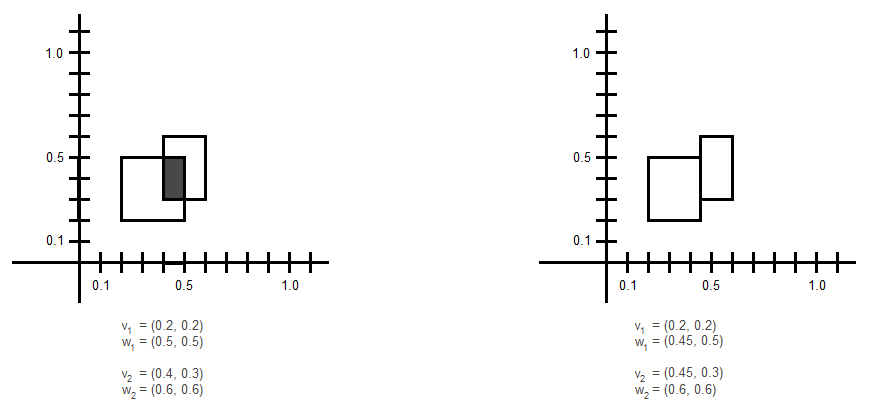
\includegraphics[width=12cm]{Immagini/elimination_overlap.png}\\
  \caption{Esempio di eliminazione di sovrapposizione}
\end{center}
\end{figure}


L'algoritmo fornisce la capacità di incorporare nuove classi e ridefinire quelle esistenti senza dover nuovamente rieffettuare il processo di apprendimento. Tuttavia, presenta anche alcune limitazioni, soprattutto nella procedura di contrazione e controllo di sovrapposizioni, comportando, negli anni, la presentazione in letteratura di nuove varianti~\cite{fmmnn_variants}. In Figura 3.4 è possibile osservane alcune, principalmente divise tra utilizzo della contrazione o meno. 

\begin{figure}[h!]
\begin{center}
  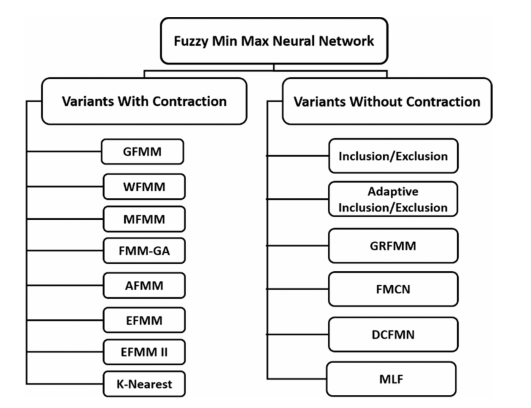
\includegraphics[width=10cm]{Immagini/varianti_FMMNN.png}\\
  \caption{Varianti dell'algoritmo FMMNN}
\end{center}
\end{figure}

Nel capitolo 4.1 si vedrà l'implementazione in Python dell'algoritmo fuzzy min-max Neural Network.

\subsection{Altre varianti}

Infine, oltre ai modelli trattati precedentemente, esistono altre possibili reti neurali fuzzy. Nella Tabella \ref{table:1} è possibile osservare una panoramica di alcuni metodi presenti in letteratura. Per comodità, alcuni metodi sono stati raggruppati per famiglia di algoritmo, di cui è fornita qui in seguito una breve elencazione delle caratteristiche più rilevanti. 

\begin{itemize}
\item \textit{Self-organizing fuzzy neural network}:  capaci di riorganizzare il modello e adattarsi a cambiamenti di \textit{environment}. Si utilizzano nuovi algoritmi di \textit{pruning}, cioè algoritmi di compressione e ottimizzazione della rete neurale. 
\item \textit{Interval Type-2 Fuzzy Neural Network}: estensione con i \textit{Type-2 Fuzzy set}, che presentano una funzione di appartenenza secondaria. Presentano una maggiore \textit{learning accuracy} con minor numero di regole rispetto al Type-1 
\item \textit{Dynamic Fuzzy Neural Network}: i neuroni posso essere ricreati o eliminati dinamicamente a seconda delle performance del sistema. L'apprendimento risulta molto più veloce. 
\end{itemize}

Interessante è anche l'algoritmo SVFNN, che combina la maggior capacità nella classificazione da parte delle support vector machine con le potenzialità già elencate delle fuzzy neural network. 


\begin{table}[h!]
\centering
\begin{tabular}{ |c|c|c|c| }
\hline
\textbf{Categoria} & \textbf{Nome metodo} & \textbf{Anno} & \textbf{ Articolo} \\
\hline
\hline
\multirow{3}{17em}{Adaptive neuro fuzzy inference system}  & ANFIS & 1993 & ~\cite{anfis} \\ 
& CANFIS-GA & 2012 & ~\cite{canfi} \\
\hline
\multirow{3}{17em}{Self-organizing fuzzy neural network} & SOFNN & 2004 & ~\cite{sofnn} \\ 
& GenSoFNN & 2002 & ~\cite{gensofnn} \\ 
& SOFNNGA & 2006 & ~\cite{SOFNNGA} \\ 
& SOFNN-IT2 & 2014 & ~\cite{sofnn-it2} \\ 
& GP-FNN & 2010 & ~\cite{GP-FNN} \\
& SOFMLS & 2009 & ~\cite{SOFMLS} \\
\hline
\multirow{3}{17em}{Interval Type-2 Fuzzy Neural Network} & SEIT2FNN & 2008 & ~\cite{SEIT2FNN} \\ 
& IT2FNN  & 2013 & ~\cite{IT2FNN} \\ 
\hline
Fuzzy min-max Neural Networks & FMMNN & 2000& ~\cite{FMMNN}\\	%era il vecchio GFMM
\hline
\multirow{3}{17em}{Dynamic Fuzzy Neural Network} & D-FNN & 2000 & ~\cite{DFNN} \\ 
& GDFNN  & 2001 & ~\cite{GDFNN} \\ 
\hline
Support-Vector-Based Fuzzy Neural Network & SVFNN & 2006 & ~\cite{SVFNN} \\
\hline
Online Self-Constructing  & SONFIN & 1998 & ~\cite{SONFIN} \\
\hline

\end{tabular}
\caption{Elenco degli algoritmi basati su reti neurali}
\label{table:1}
\end{table}

\clearpage


\section{ K-Nearest Neighbour}	
L'algoritmo nearest neighbour è uno degli algoritmi più semplici e facili da implementare nell'apprendimento automatico supervisionato. Vede le sue applicazioni principali nei problemi di classificazione e di regressione. L'idea basilare di questo algoritmo è che due oggetti, se sono simili, saranno vicini tra loro. Si consideri l'insieme $X={x_1, x_2, ..., x_n}$ di n campioni etichettati e si ponga $x_j \in X$ come l'esempio più vicino ad $x$. L'algoritmo classificherà $x$ con la stessa etichetta associata a $x_j$. L'algoritmo può essere esteso come  K-nearest neighbor, che classifica un oggetto con la stessa etichetta rappresentata dalla maggioranza dei $k$ campioni più vicini. Durante la fase di apprendimento, occorre partizionare lo spazio in diverse regioni, in riferimento alle feature e alle posizioni che occupano gli esempi di apprendimento. Fissato il parametro $k$, corrispondente al numero di vicini necessari per decretare l'etichetta di un oggetto, si andranno a calcolare le distanze tra l'oggetto da classificare e tutti i punti dello spazio, corrispondenti agli esempi di apprendimento. Per calcolare la distanza, si può utilizzare la distanza euclediana, molto utile se le variabili sono dello stesso tipo:

$$d\left( p,q\right)   = \sqrt {\sum _{i=1}^{n}  \left( q_{i}-p_{i}\right)^2 }$$

oppure, la distanza di Manhattan, utile se le variabili non sono dello stesso tipo:


$$  d\left( p,q\right) = |x_{p}-x_{q}|+|y_{p}-y_{q}| $$


o, se si opera con stringhe, si può utilizzare la distanza di Hamming. 
Una volta calcolata la distanza tra l'oggetto da classificare e tutti i punti dello spazio, le si elencano in ordine non decrescente e si selezionano i primi $k$ punti più vicini. Infine, verrà attribuita all'oggetto l'etichetta più frequente nei $k$ punti più vicini selezionati. 
Un esempio grafico del k-Nearest Neighbour è presente in Figura 3.5. 

\begin{figure}[h!]
\begin{center}
  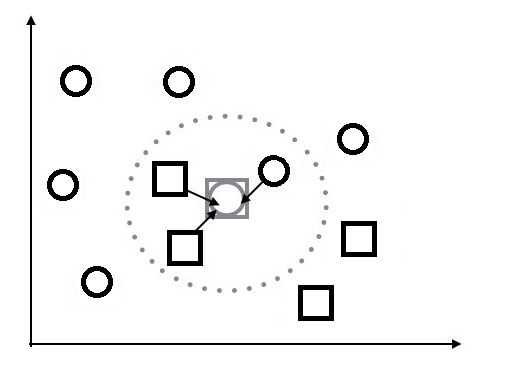
\includegraphics[width=10cm]{Immagini/KNN.png}\\
  \caption{Esempio di k-Nearest Neighbour con $k$ pari a 3}
\end{center}
\end{figure}

Tra i vantaggi dell'algoritmo KNN si possono annoverare la sua estensibilità a molti problemi, l'alta accuratezza e semplicità di implementazione e l'adattabilità sui dati. Infatti, l'algoritmo non è parametrico e dunque non viene fatta assunzione sui dati, ma il modello viene costruito interamente dai dati forniti. Tuttavia, l'algoritmo diventa computazionalmente costoso all'aumentare delle dimensioni del dataset, dal momento che conserva la maggior parte dei dati. Ciò comporta tempi cospicui nel dover processare un dataset di grandi dimensioni. Un modo per migliorare le performance dell'algoritmo può essere fare \textit{feature selection}, di modo da ridurre il numero di attributi irrilevanti ai fini della classificazione. Un'altra questione delicata è decretare il valore del parametro $k$, in base al quale può variare sensibilmente l'esito della classificazione. Per maggiori chiarimenti, si rimanda al Capitolo 4.2

\subsection{Fuzzy k-Nearest Neighbour}

\`E possibile coniugare l'algoritmo k-Nearest Neighbour alla logica fuzzy, ottenendo così il \textit{Fuzzy K-Nearest Neighbour}. Questo algoritmo, a differenza della versione base, non assegnerà la classe all'oggetto, ma computerà i gradi di appartenenza a tutte le classi possibili, per evitare nessuna assegnazione arbitraria. I gradi di appartenenza assegnati dipendono dalla distanza dell'oggetto dai k campioni più vicini e dai gradi di appartenenza di quest'ultimi dalle classi possibili. Infatti, uno dei problemi della versione base dell'algoritmo è che i campioni vengono considerati allo stesso modo importanti nell'assegnamento dell'etichetta all'oggetto in questione. Ciò genera spesso difficoltà laddove vi siano sovrapposizioni di campioni. Pertanto in generale, la versione fuzzy consente di poter definire il grado di appartenenza di un oggetto in una certa classe, in base alla quale ridefinire l'importanza dei campioni vicini nel determinare la classe ed evitare situazioni ambigue. Infatti, avere dei gradi di appartenenza permette di poter definire con maggior sicurezza l'appartenenza o meno di un oggetto a una classe e, dunque, consente di aver maggiore sensibilità nella classificazione. Ad esempio, se un oggetto viene assegnato con un grado di appartenenza pari a 0.9 a una classe e 0.05 a un'altra, sarà altamente probabile che l'oggetto appartenga alla prima classe; d'altra parte, se un oggetto ha un grado di appartenenza pari a 0.55 a una classe e un 0.44 a un'altra, allora l'esito della classificazione sarà un po' più incerto. In tal caso allora sarà necessaria maggiore attenzione e magari una seconda esaminazione, per comprendere quale delle due classi sia eventualmente la più consona. Grazie all'implementazione fuzzy, pertanto, si raffina la classificazione. L'algoritmo fuzzy è simile alla versione crisp, dalla quale differisce dopo aver selezionato i $k$ campioni più vicini. 

Nel Capitolo 4.2 si vedrà l'implementazione in Python del Fuzzy K-Nearest Neighbour. 


\subsection{Varianti}

Il Fuzzy K-Nearest Neighbour, tuttavia, presenta alcune debolezze che hanno portato a ricercare varianti per poterle affrontare al meglio. Molte ricerche hanno proposto varie tecniche, tra le quali l'uso della riduzione dei dati, sviluppo di metodi per decretare l'iperparametro $k$, introduzione dei pesi per adattare l'influenza delle feature e versioni più velocizzate per la ricerca dei campioni più vicini. 

In particolare, esiste un'estenzione ai fuzzy rough set, che introduce la cosiddetta \textit{classificazione possibilistica}. Infatti, un algoritmo di classificazione dovrebbe notificare la situazione in cui un oggetto non appartiene in realtà a nessuna classe: tale abilità è, difatti, alla base della mente umana, che è in grado di cogliere la non-appartenenza di un oggetto a tutte le classi da lui apprese con l'esperienza. Ad esempio, se un essere umano conosce solo cerchi e rettangoli e gli viene presentato un triangolo, egli sarà in grado di affermare che tale oggetto non apparterrà a nessuna classe da lui conosciuta. L'algoritmo FKNN in generale non possiede questa caratteristica. Si introduce dunque il FRNN, in cui, invece di considerare i $k$ campioni più vicini come punti di riferimento, comprende tutti i campioni dello spazio, assegnando gradi di appartenenza diversi. In questo modo, non si presenta il problema di scegliere il valore ottimale di $k$. 

Tra le varianti, è possibile ritrovare nuovamente l'estensione ai Type-2 fuzzy set (si veda il IT2FKNN). Sono presenti anche modalità ibride del Fuzzy-KNN, combinato con algoritmi genetici (GAFuzzyKNN) e clustering (FCMKNN), che consentono di combinare i punti di forza di entrambi gli algoritmi. 

In generale, in Tabella \ref{table:2} è possibile osservare una panoramica di alcuni metodi presenti in letteratura. Per comodità, alcuni metodi sono stati raggruppati per famiglia di algoritmo. Si annoverano le seguenti categorie: 

\begin{itemize}
\item \textit{Interval-valued fuzzy set k-NN}: i valori di membership di ogni campione di training vengono rappresentati come array di intervalli, restituendo una rappresentazione più flessibile della tipicità delle istanze per ogni classe del problema. Usando questo approccio, si riduce sensibilmente la dipendenza al parametro $k$ del FKNN. 
\item \textit{Intuitionistic k-Nearest Neighbour}: utilizzo di intuitionistic set, che sono un'estensione dei fuzzy set classici. Introduce il concetto di grado di non-appartenenza. Dagli esperimenti, si ottiene un'accuratezza lievemente superiore. 
\item \textit{Possibilistic k-Nearest Neighbour}: introduzione della teoria della possibilità, per gestire in maniera più ottimale rappresentazioni di incertezza. 
\item \textit{Preprocessing Methods via Data Reduction}: lavori di preprocessing al dataset, prima o dopo aver effettuato il processo di training, per diminuire i costi computazionali. Ad esempio, si possono introdurre set di classi prototipo, oppure applicare algoritmi di \textit{pruning}.
\end{itemize}

Infine, un algoritmo recente, molto interessante e che riassume i punti di forza dei metodi presentati in questa tesi è il FNNP, che combina le reti neurali e il FKNN.~\cite{FKNN-NN}

\begin{table}[h!]
\centering
\begin{tabular}{ |c|c|c|c| } 
\hline
\textbf{Categoria} & \textbf{Nome metodo} & \textbf{Anno} & \textbf{Articolo} \\
\hline
\hline
\multirow{3}{17em}{Fuzzy set k-Nearest Neighbour}  & FKNN & 1985 & ~\cite{FKNN} \\ 
& VWFuzzyKNN & 1999 & ~\cite{VWFuzzyKNN} \\
& FCMKNN & 1986 & ~\cite{FCMKNN} \\
& GAFuzzyKNN & 2005 & ~\cite{GAFuzzyKNN} \\
& LPKNN & 2011 & ~\cite{LPKNN} \\
\hline
Fuzzy-rough set k-Nearest Neighbour & FRNN & 2011 & ~\cite{FRNN} \\ 
\hline
\multirow{3}{17em}{Interval-valued fuzzy set k-NN} & IV-kNN  & 2015 & ~\cite{IV-KNN} \\ 
& EF-kNN-IVFS  & 2014 & ~\cite{EF-KNN-IVFS} \\ 
\hline
Type-2 Fuzzy Set k-Nearest Neighbour & IT2FKNN & 2003 & ~\cite{IT2FKNN}\\
\hline
\multirow{3}{17em}{Intuitionistic k-Nearest Neighbour} & IFVKNN & 1998 & ~\cite{IFSKNN} \\ 
& IF-KNN & 1995 & ~\cite{IF-KNN} \\ 
& IFV-NP & 2001 & ~\cite {IF-KNN}\\
\hline
\multirow{3}{17em}{Possibilistic k-Nearest Neighbour} & D-SKNN  & 2002 & ~\cite{D-SKNN} \\ 
& poSIBL  & 2002 & ~\cite{D-SKNN} \\ 
\hline
Modified Fuzzy k-Nearest Neighbour & MOGA-MFNN & 2017 & ~\cite{ MOGA-MFNN} \\
\hline
\multirow{3}{17em}{Preprocessing Methods via Data Reduction} & PFKNN & 2009 & ~\cite{PFKNN} \\
& FuzzyNPC & 1985 & ~\cite{FKNN} \\
& FENN & 1998 & ~\cite{FENN} \\
\hline
Parameter independent fuzzy weighted & PIFW-kNN & 2017 & ~\cite{PIFW-kNN} \\
\hline
\end{tabular}
\caption{Elenco degli algoritmi basati su  k-Nearest Neighbour}
\label{table:2}
\end{table}

\clearpage

% POSSO CITARE https://www.researchgate.net/publication/335634726_An_Improved_Neural_Network_Classifier_Using_Fuzzy_Nearest_Neighbor_Partitioning_Method CHE COMBINA RETI NEURALI E FKNN

	\chapter{Implementazioni ed esperimenti}
	\section{Algoritmi basati su reti neurali}
	\section{Algoritmi basati su k-Nearest neighbour}

%The algorithm does not generate smooth membership curves in overlapping regions. Può essere utile dopo, ho notato una cosa nelle visualizzazioni della membership

%RICORDA di parlare della scelta di k!!! C'è un po' da dire, illustrare come influenza. Cose da dire (da sistemare e cercare altre fonti): ARTICOLO 2!!! The value of K implicitly indicates the space of the neighborhood around the test pattern. When K is one, the
%class label of the test pattern is determined just based on the class label of the closest neighbor. This scheme suffers if the class label of the closest neighbor is corrupted by noise. On the other hand, when K is equal to the total number of the training patterns, the information becomes too global, and the class label of the test pattern is determined based on the a priori probability of the classes. The large value of K may increase the classification efficiency as there are more bodies of evidence to classify the test pattern. But if the neighborhood is large, then the neighbors may belong to more than one class. It happens especially in the region where two classes overlap, or noise is present. Thus, it may increase the confusion in assigning the class label to the test pattern. Therefore, the optimal value of K can only be found by a trade-off, which is currently achieved using trial and error procedures. 

%Illustrare lo pseudocodice 
% 

	\subsection{Risultati}
	\chapter{Conclusioni}


\bibliographystyle{ieeetr}
\bibliography{bibliografia}

\end{document}